\documentclass{beamer}

\usepackage{amssymb,amsthm,amsmath} %ams
\usepackage[finnish]{babel} %suomenkielinen tavutus
\usepackage[T1]{fontenc} %skanditavutus
\usepackage[utf8x]{inputenc}        	% skandit utf-8 koodauksella
\usepackage{graphicx}
\usepackage{tikz}% vähän tehokkaampi grafiikkapaketti
\usepackage[square]{natbib}

\begin{document}

\frame{
 \frametitle{Avaruusjakoon perustuvat tietorakenteet tietokonegrafiikassa}
 %\framesubtitle{}
}

\frame{
 \frametitle{Mitä kandidaatintutkielmani käsittelee}
 %\framesubtitle{}
}

\frame{
 \frametitle{Käsitteitä}
  \begin{itemize}
   \item{\textbf{\emph{hahmontaminen}} (engl. \emph{rendering}): luo kolmiulotteisesta maisemasta kaksiulotteisen kuvan}

   \item{\textbf{\emph{maisema}} (engl. \emph{scene}): joukko geometrisesti määriteltyjä \emph{objekteja}, esimerkiksi hahmo, rakennus, puu..., ja valonlähteitä}

   \item{\textbf{\emph{monikulmio}} (engl. \emph{polygon}): objektit on usein jaettu pienempiin osiin, useimmiten kolmioihin hahmontamisen helpottamiseksi}

   \item{\textbf{\emph{säteenseuranta}} (engl. \emph{ray tracing}): hahmontamistekniikka, joka mallintaa valonsäteiden kulkua maisemassa. Tuottaa erittäin realistisia kuvia}
  \end{itemize}
}

\frame{
 \frametitle{Käsitteitä}
 %\framesubtitle{}
 \begin{figure}
  \centering 
  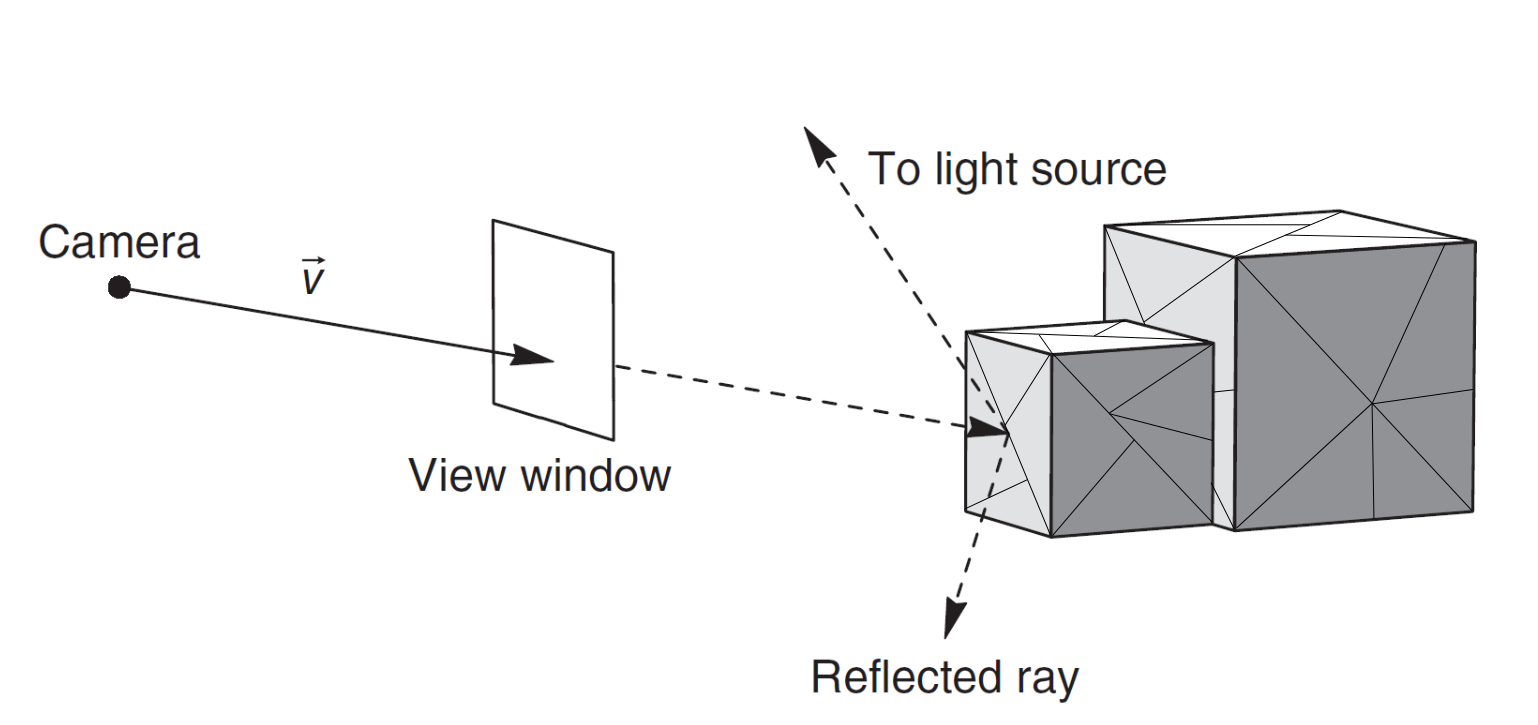
\includegraphics[width=0.8\textwidth]{img/raytracingtri.png}
  \caption{Säteenseuranta \citep{janke}}
  \label{raytracing}
  \vspace{-0.5cm}
 \end{figure}
}


\frame{
 \frametitle{Säteenseuranta on hidasta}
 %\framesubtitle{}
}

\frame{
 \frametitle{BSP-puu}
 %\framesubtitle{}
}

\frame{
 \frametitle{kd-puu}
 %\framesubtitle{}
}

\frame{
 \frametitle{Rajaavat tilat}
 %\framesubtitle{}
}

\frame{
 \frametitle{Tietorakenteiden alustamisen vertailua}
 %\framesubtitle{}
}

\frame{
 \frametitle{Tietorakenteiden käytön vertailua}
 %\framesubtitle{}
}

\frame{
 \frametitle{Reaaliaikainen säteenseuranta}
 %\framesubtitle{}
}

\bibliographystyle{apalike-finnish} %apalike-finnish
\bibliography{bibliography}

\end{document}
